\chapter{Drone flight measuring test}\label{ap:drone_flight_test}
The purpose of this test is to get a model of how the drone are moving in upward movements, and to make a function of the behaviour. The test will be performed in the Motion detection Lab, located in room  at AAU, where the Vicon system  is placed. The reason for using this system is because it can track an object's position in all x, y and z-axis at the same time. From this data it will be possible to make a model of the drone's movements and from that make the transfer function.

\section*{Test setup}
The components there are used in the test are as the following point:
\begin{itemize}
    \item{Vicon system}
    \item{Reflectors}
    \item{Drone}
    \item{Teensy 3.2} % navnet på micro kontrolene
    \item{Turnigy TGY-iA6} % navn på reciver
    \item{Turnigy TGY-A6} % navn på transmitter
\end{itemize}
For the Vicon tracking system to track the drone, five reflectors is set on the drone. The placement of the reflectors can be seen in figure \ref{fig:reflectors}.
The drone are placed in the room with the Vicon cameras. Where the Vicon system can record the drones movement, by tracking the reflectors. 

\begin{figure}[H]
    \centering
    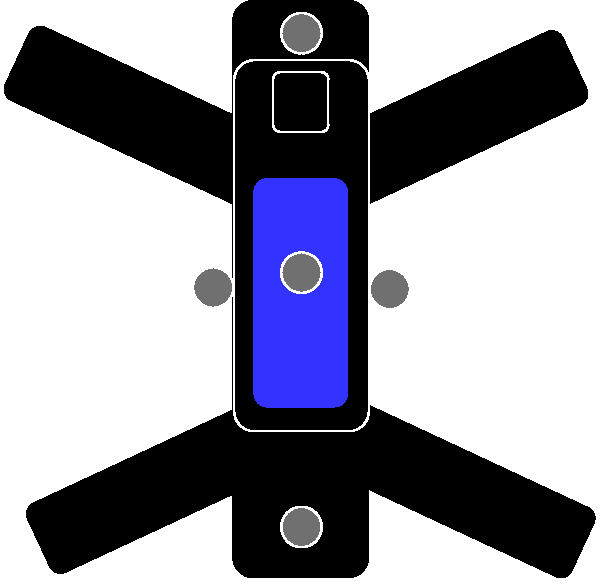
\includegraphics[width=0.4\textwidth]{figures/Appendix/measuringTest/Reflector1.pdf}
    \caption{Illustration of placement of the reflectors on the drone}
    \label{fig:reflectors}
\end{figure}


\section*{Execution}
rBefore the test can be executed, a calibration of the Vicon cameras have to be done. After the Calibration the test code are transferred to the Teensy for controlling the drone. When the Vicon system is set to track the drone by it's reflectors, the drone is then set to fly at a steady level. From this steady level, it is set to run a program, which makes the drone keep a throttle level on 30 \% in 10 seconds, and then raise the level to 33\% in 1 second and then back to 30\% afterwards. The code to run this program can be seen in the Github repository. From this step response it is possible to make a model of the drones movements, and calculate the values for the transfer function. 



\section*{Results}
The data is plotted in the figure \ref{}, in this figure the plot is directly from the data, which is time and position. In the figure the blue line is the plotted data.

\begin{figure}[H]
    \centering
    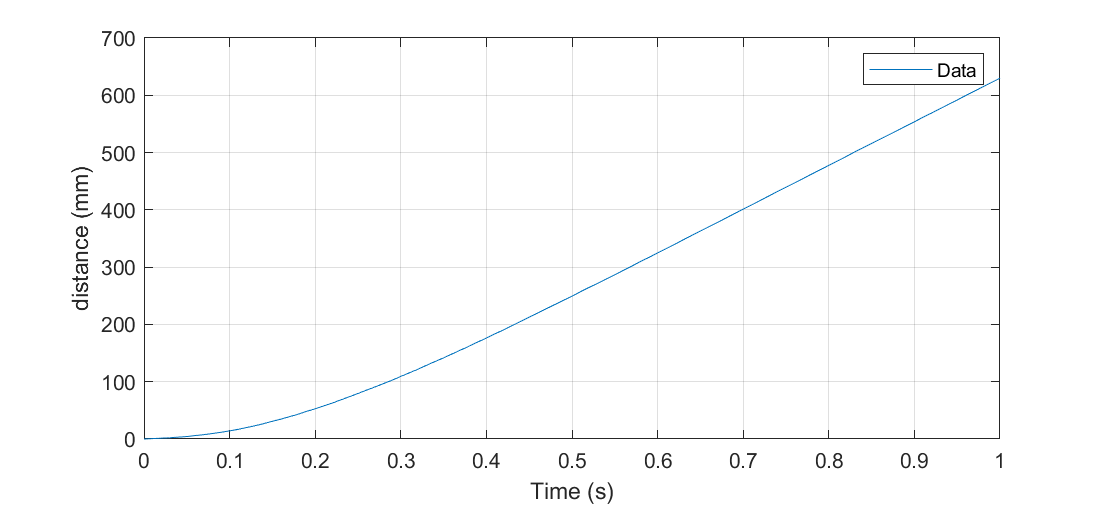
\includegraphics[width=\textwidth]{figures/Appendix/measuringTest/DroneTest.png}
    \caption{Plot of the data }
    \label{fig:positiontime}
\end{figure}

\section*{Discussion}
From these two data plots,



\section*{Conclusion}
